\begin{scriptsize}
  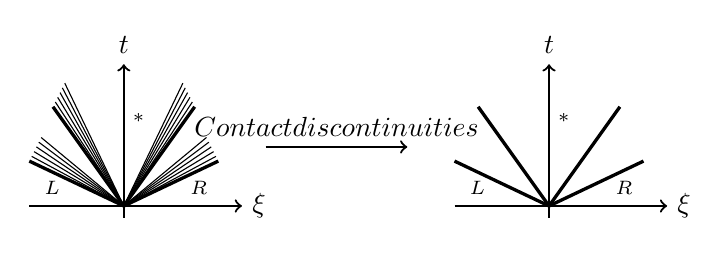
\begin{tikzpicture}[scale=0.3]
    \draw[->,thick] (-4,0) -- (5,0) node [right] {$\xi$};
    \draw[->,thick](0,-0.5) -- (0,6) node [above] {$t$};
    % Fastest left
    \draw[very thick](0,0) -- (-4,1.9) ;
    \draw(0,0) -- (-3.9,2.1) ;
    \draw(0,0) -- (-3.8,2.3) ;
    \draw(0,0) -- (-3.7,2.5) ;
    \draw(0,0) -- (-3.6,2.7) ;
    \draw(0,0) -- (-3.5,2.9) ;
    % Slowest left
    \draw[very thick](0,0) -- (-3.,4.2) ;
    \draw(0,0) -- (-2.9,4.4) ;
    \draw(0,0) -- (-2.8,4.6) ;
    \draw(0,0) -- (-2.7,4.8) ;
    \draw(0,0) -- (-2.6,5.0) ;
    \draw(0,0) -- (-2.5,5.2) ;
    % Fastest right
    \draw[very thick](0,0) -- (4,1.9) ;
    \draw(0,0) -- (3.9,2.1) ;
    \draw(0,0) -- (3.8,2.3) ;
    \draw(0,0) -- (3.7,2.5) ;
    \draw(0,0) -- (3.6,2.7) ;
    \draw(0,0) -- (3.5,2.9) ;
    % Slowest right
    \draw[very thick](0,0) -- (3.,4.2) ;
    \draw(0,0) -- (2.9,4.4) ;
    \draw(0,0) -- (2.8,4.6) ;
    \draw(0,0) -- (2.7,4.8) ;
    \draw(0,0) -- (2.6,5.0) ;
    \draw(0,0) -- (2.5,5.2) ;
    \node(a) at (-3,0.75) {$\Ucb_L$};
    \node(b) at (3.2,0.75) {$\Ucb_R$};
    \node(c) at (0.65,3.5) {$\Ucb^*$};
    \draw[->,thick](6.,2.5)--(12.,2.5) node[above,midway] {$\text{Contact discontinuities}$};
    \begin{scope}[shift={(18.,0.)}]
      \draw[->,thick] (-4,0) -- (5,0) node [right] {$\xi$};
      \draw[->,thick](0,-0.5) -- (0,6) node [above] {$t$};
      % Fastest left
      \draw[very thick](0,0) -- (-4,1.9) ;
      % Slowest left
      \draw[very thick](0,0) -- (-3.,4.2) ;
      % Fastest right
      \draw[very thick](0,0) -- (4,1.9) ;
      % Slowest right
      \draw[very thick](0,0) -- (3.,4.2) ;
      \node(a) at (-3,0.75) {$\Ucb_L$};
      \node(b) at (3.2,0.75) {$\Ucb_R$};
      \node(c) at (0.65,3.5) {$\Ucb^*$};
    \end{scope}
  \end{tikzpicture}
\end{scriptsize}

%%% Local Variables:
%%% mode: latex
%%% TeX-master: "../../presentation"
%%% End: